% !TeX root = ../main.tex

\chapter{实验评估}

截止至论文完成前,项目仍在进行中,以下内容只介绍了目前取得的部分实验结果,并对实验结果简要分析。

\section{实验环境}
实验平台基于Intel Xeon家族的第三代处理器,详细如下表所示:

\begin{table}[htb]
  \centering\small
  \caption{实验环境}
  \label{tab:ex1}
  \begin{tabular}{p{90pt}p{180pt}}
    \toprule
    项目    & 内容\\
    \midrule
    处理器  &  Xeon(R) CPU E5-2690 v3 x24 \\
    内存    &  64GB\\
    操作系统&  Ubuntu 16.04  \\
    编程语言&  C++14\\
    跨机器网络延迟 & <1ms\\

    \bottomrule
  \end{tabular}
\end{table}

\section{性能评价标准}
为了进行系统复现,并比较不同系统之间的性能,采用了上一章节介绍的TPC-C和Retwis工作负载,同时为了提供除去并发控制协议和共识协议之外,其余系统实现部分对于性能的影响,我们采用了一个完全随机读写的工作负载,在该工作负载中,我们将所有实现的系统与不实现并发控制的方案相比较,从而观察在低冲突概率下,并发控制对系统的性能影响。

系统的发展历经数十年风雨,人们通常以时延(latency)和吞吐量(throuhhput)作为评价指标,但是时延包括了很多中计算方式。随着服务器性能的不断提高,人们意识到系统的尾部时延更能反应系统的公平性和优越性,例如99th 时延。同时,作为事务处理系统,事务的放弃率(abort rate)也是衡量系统的重要标准,一个放弃率很高的系统,会导致用户的反复重试(retry)从而毒害系统的性能。

因此,我们采用以下评价指标作为衡量标准:


\begin{itemize}
\item 系统的聚合吞吐量
\item 99th latency
\item 放弃率(Abort rate)
\end{itemize}

同时我们将通过zipf系数来调整不同的冲突概率,用于验证不同系统在不同冲突概率下的表现。运行TPC-C\cite{TPCC}、RW、TPC-A(zipf)\cite{TPCA}、Retwis 工作负载。
\section{单数据中心测试}
该实验模拟了在同一个数据中心内的不同系统性能之间的表现,由于相关工作中介绍的系统大多为了异地环境所设计,虽然同一数据中心属于该范围的子集,但他们大多针对异地环境做了优化。而本实验将研究他们在同一个数据中心内的表现。

为了模仿单数据中心,我们不需要在服务器中间添加任何流量控制策略。

\paragraph{RW测试负载}
在RW测试中,我们采用了900个客户端,此时系统能够达到一个比较好的吞吐量,再额外增加会大大增加时延,却贡献了很少的吞吐量。在该配置下,Janus可以达到16w+的吞吐量(tps),而Tapir达到了23w+的吞吐量。这和我们的预期一致,在低冲突概率的条件下,Tapir依赖的OCC协议可以很好的工作,而Janus因为其依赖的图计算方式,给系统性能带来了一定的损失。

\paragraph{TPC-A zipf实验}
在该实验中我们调整事务之间的冲突概率,观察不同系统的性能随着冲突概率的变化而变化的趋势。

从实验结果可以看出,在较高冲突概率下,与RW测试相反,Janus具有比Tapir更高的吞吐量,并且Tapir随着冲突概率的进一步提高,吞吐量降低。Janus则基本维持不变,同样的,这一信息也在提交率上体现,Jasnus始终维持的100\%的提交率,Tapir的提交率在zipf系数为1时,却接近于0。见图~\ref{fig:pic1}和~\ref{fig:pic2}


\paragraph{TPC-C 实验}
TPC-C可以被视作是一个冲突率较高的负载,同时,其模拟仿真了真实的商业环境,因此,具有一定的现实指导意义。实验结果如~\ref{fig:pic3}、~\ref{fig:pic4}和~\ref{fig:pic5}所示,其中横坐标采用的客户端数量取log。

从实验结果可以看出Tapir在低负载的情况下表现的更好,具有较高的吞吐量和较高的提交率,但Janus在高并发(高负载)的情况下,表现更出色,因为此时Tapir因为其过高的失败率而阻碍了系统性能。

\begin{figure}[htb]
  \centering
  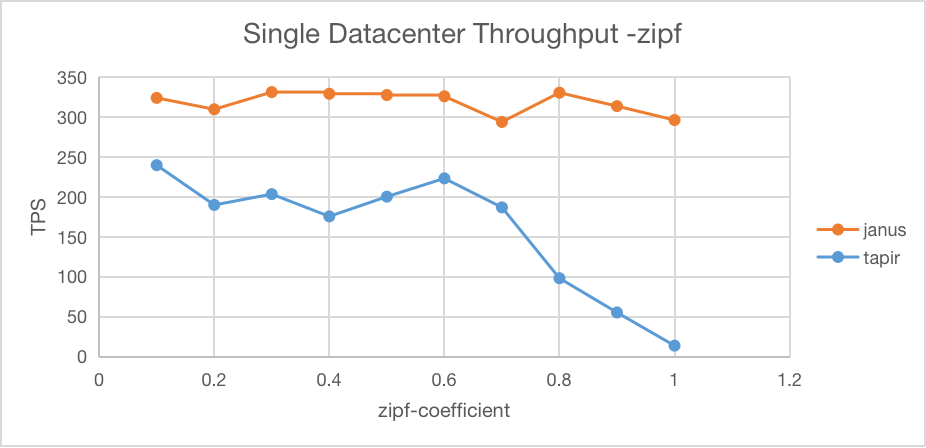
\includegraphics[width=0.8\textwidth]{Picture1.png}
  \caption{单数据中心 TPCA-zipf 吞吐量测试}
  \label{fig:pic1}
\end{figure}


\begin{figure}[htb]
  \centering
  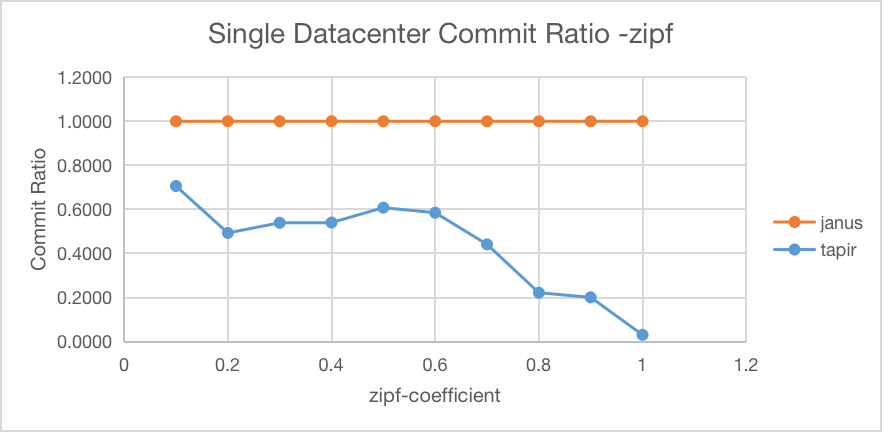
\includegraphics[width=0.8\textwidth]{Picture2.png}
  \caption{单数据中心 TPCA-zipf 提交率测试}
  \label{fig:pic2}
\end{figure}

\begin{figure}[htb]
  \centering
  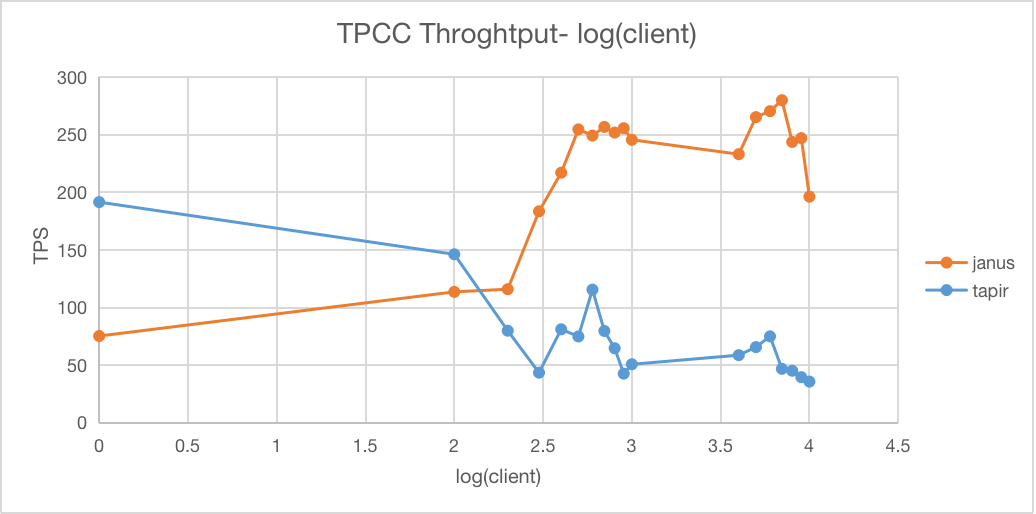
\includegraphics[width=0.8\textwidth]{Picture3.png}
  \caption{单数据中心 TPCC 吞吐量测试}
  \label{fig:pic3}
\end{figure}

\begin{figure}[htb]
  \centering
  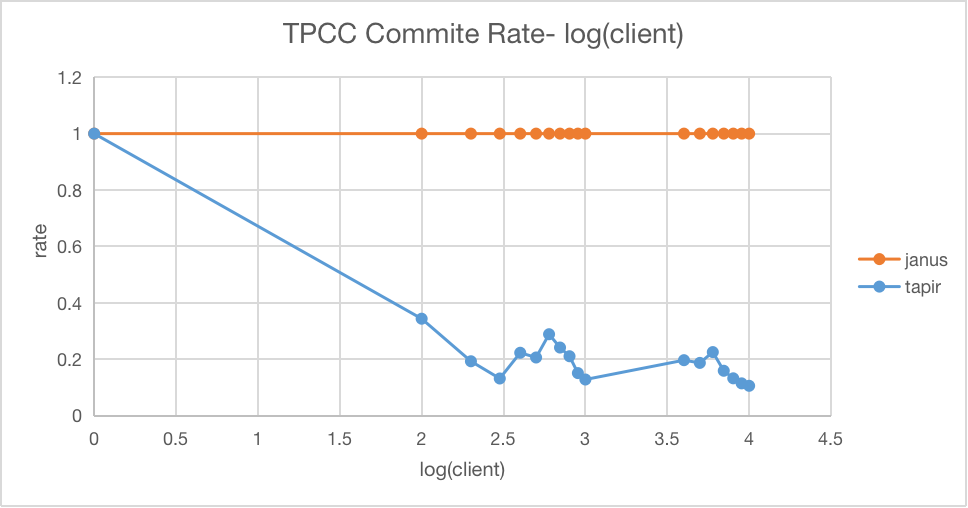
\includegraphics[width=0.8\textwidth]{Picture4.png}
  \caption{单数据中心 TPCC 提交率测试}
  \label{fig:pic4}
\end{figure}

\begin{figure}[htb]
  \centering
  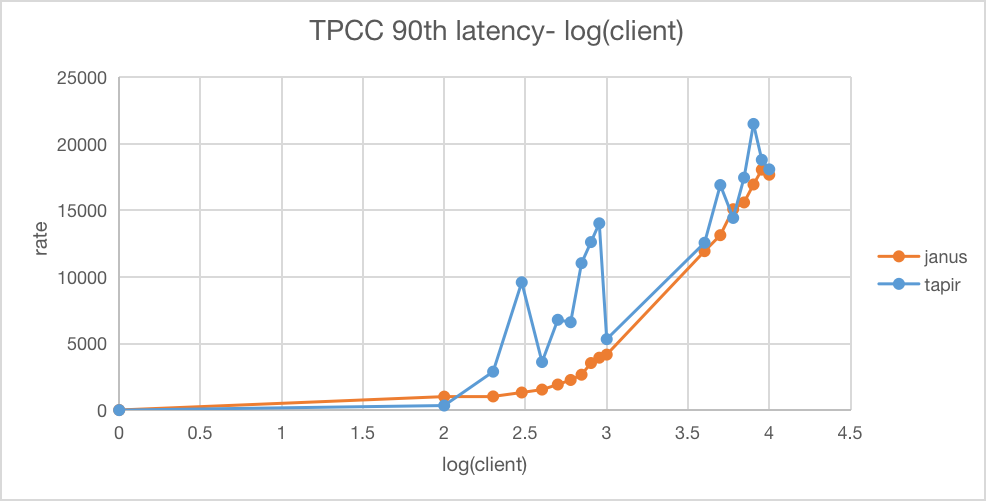
\includegraphics[width=0.8\textwidth]{Picture5.png}
  \caption{单数据中心 TPCC 时延测试}
  \label{fig:pic5}
\end{figure}

\section{异地多数据中心测试}
为了在我们的服务器集群中,模仿异地跨数据中心的实现,我们通过在服务器中间添加流量控制(Traffic Control)来实现。使用ubuntu的流量控制工具,我们可以给我们的服务器之间添加时延和波动,这里的流量控制是根据IP绑定的,因此可以在不同的服务器之间设置不同的时延。

以下是我们采用的是延信息:

\begin{table}[htb]
  \centering\small
  \caption{PING时延}
  \label{tab:ex1}
  \begin{tabular}{p{90pt}p{90pt}p{90pt}p{90pt}}
    \toprule
        & 机器 1&机器2&机器3 \\
    \midrule
    机器1&  0.064&91.7&188 \\
    机器2&  &0.063&253\\
    机器3&  & &0.064  \\

    \bottomrule
  \end{tabular}
\end{table}

同样的,我们测试不同系统在RW、TPC-A zipf、TPC-C下的表现。

\begin{figure}[htb]
  \centering
  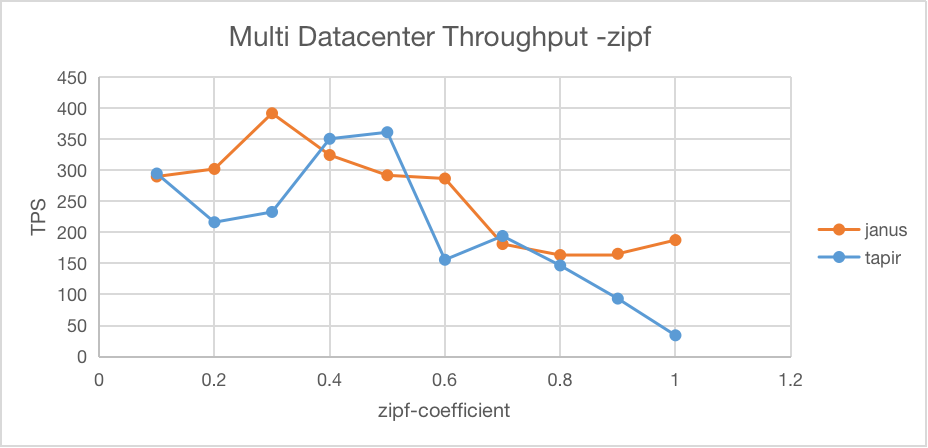
\includegraphics[width=0.8\textwidth]{Picture6.png}
  \caption{多数据中心 TPCA-zipf 吞吐量测试}
  \label{fig:pic6}
\end{figure}


\begin{figure}[htb]
  \centering
  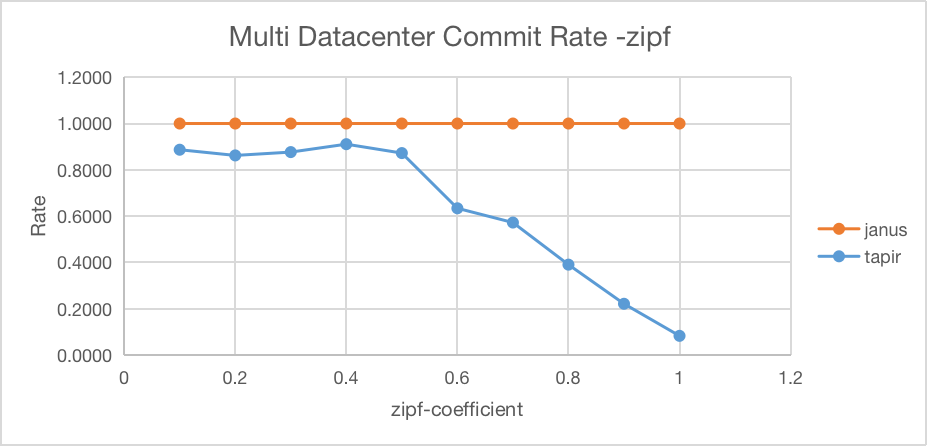
\includegraphics[width=0.8\textwidth]{Picture7.png}
  \caption{多数据中心 TPCA-zipf 提交率测试}
  \label{fig:pic7}
\end{figure}

\begin{figure}[htb]
  \centering
  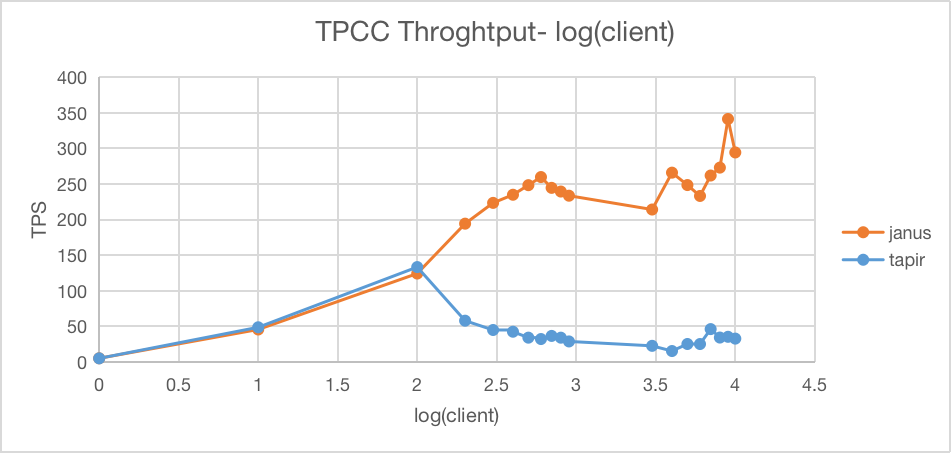
\includegraphics[width=0.8\textwidth]{Picture8.png}
  \caption{多数据中心 TPCC 吞吐量测试}
  \label{fig:pic8}
\end{figure}

\begin{figure}[htb]
  \centering
  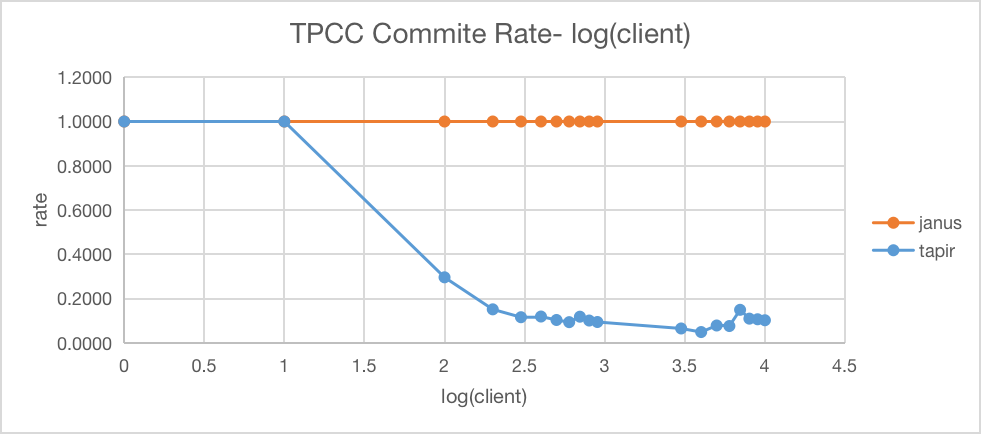
\includegraphics[width=0.8\textwidth]{Picture9.png}
  \caption{多数据中心 TPCC 提交率测试}
  \label{fig:pic9}
\end{figure}

\begin{figure}[htb]
  \centering
  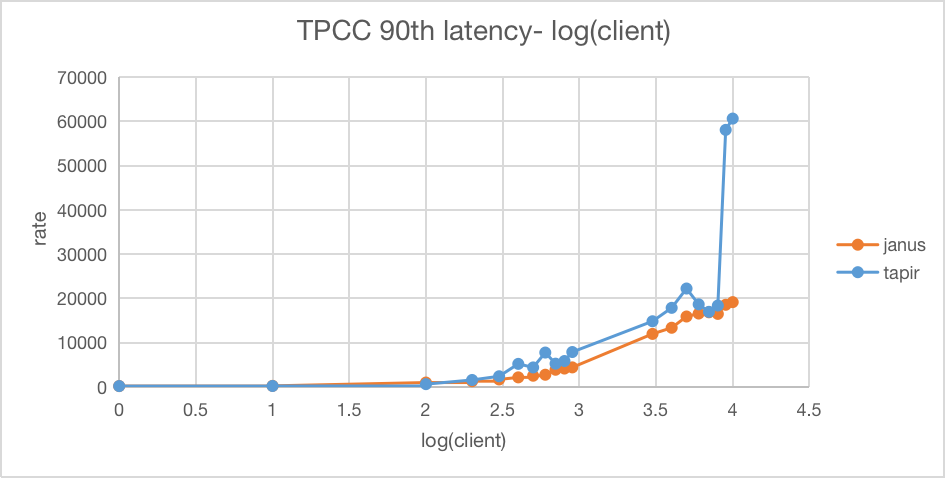
\includegraphics[width=0.8\textwidth]{Picture10.png}
  \caption{多数据中心 TPCC 时延测试}
  \label{fig:pic10}
\end{figure}

\section{部分冗余测试}

有些系统在数据中心拥有所有shard的时候拥有更好的表现,例如Janus,在全备份的情况下,只需要在同一个数据中心内询问其余碎片的执行情况,而不需要引入跨数据中心的RTT。因此,本实验希望了解在部分冗余的场景下,对这些系统的性能的影响,从而进一步了解这些系统存在的不足和缺陷。见~\ref{fig:pic11}、~\ref{fig:pic12}。


可以看出部分冗余环境下,Janus和Tapir的性能都受到了不小的影响,且Janus受到的影响更大。


\begin{figure}[htb]
  \centering
  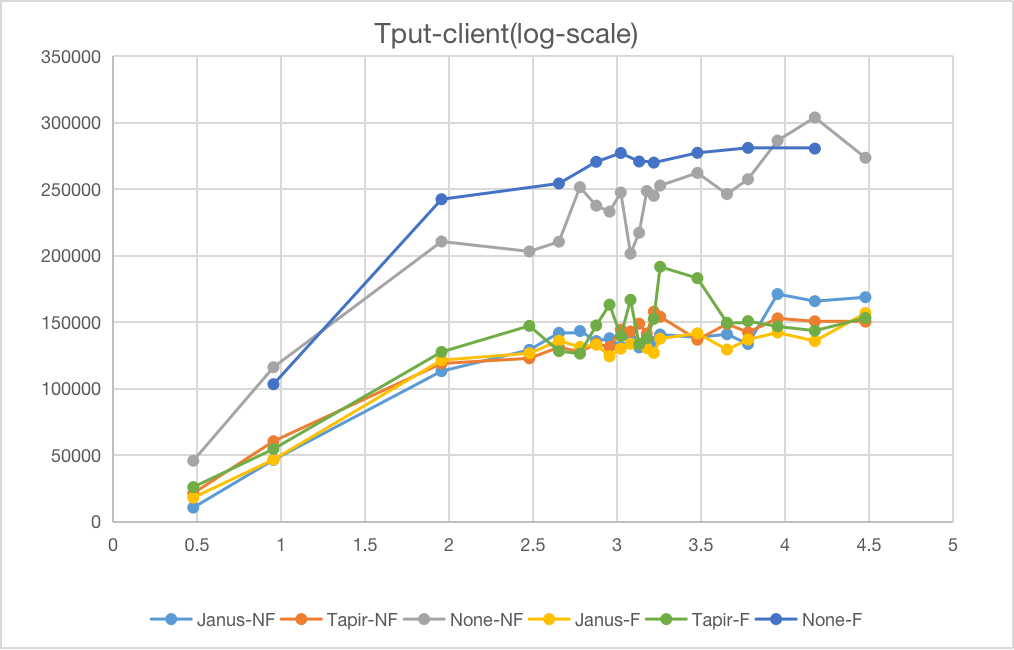
\includegraphics[width=1\textwidth]{Picture11.png}
  \caption{部分冗余的RW 吞吐量测试}
  \label{fig:pic11}
\end{figure}

\begin{figure}[htb]
  \centering
  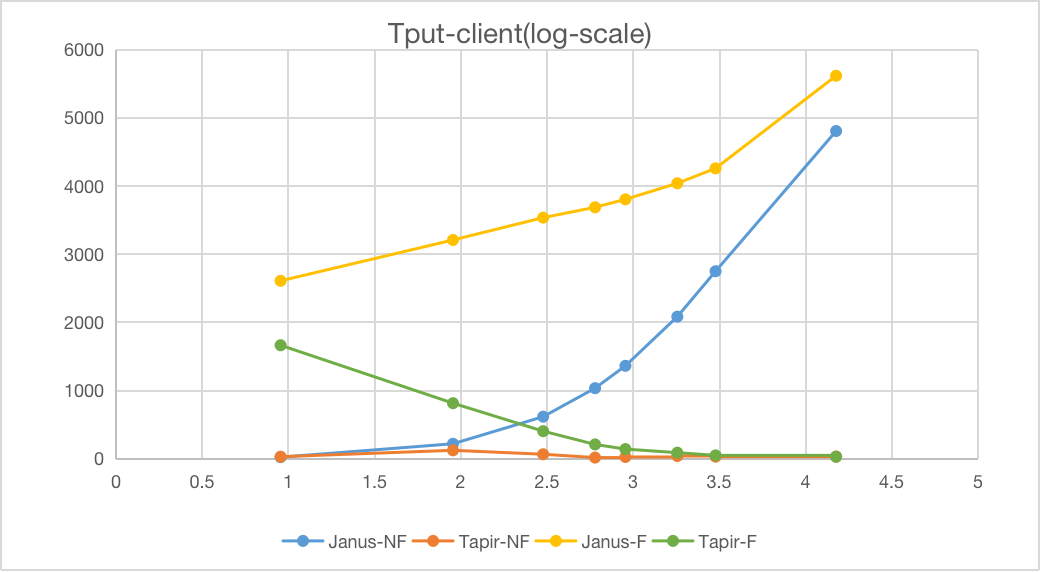
\includegraphics[width=1\textwidth]{Picture12.png}
  \caption{部分冗余的TPC-C 吞吐量测试}
  \label{fig:pic12}
\end{figure}




